\documentclass[11pt, fleqn]{article}

\usepackage{amsmath}
\usepackage{amsfonts}
\usepackage{amsthm}
\usepackage[margin=1in]{geometry} % To set the margin widths
\usepackage{graphicx}
%\usepackage{hyperref}
\usepackage{listings}
\usepackage{multirow}
\usepackage{tabularx}
\usepackage{varioref}
\usepackage{cleveref}  % this redefines vref to use cleverref
\usepackage{siunitx}
%\usepackage{subcaption}
\usepackage{subfig}
\usepackage{titlesec}
\usepackage{bm}

\crefname{equation}{equation}{equations}
\crefname{figure}{figure}{figures}

\sisetup{output-exponent-marker=\textsc{e}}

\titleformat{\section}[block]{\bfseries}{\thesection}{1em}{}


\setlength{\parskip}{12pt} % Sets a blank line in between paragraphs
\setlength\parindent{0pt} % Sets the indent for each paragraph to zero

\begin{document}

\title{Big Data: Homework 4}
\author{Will Clark \& Matthew DeLio \\ 41201-01}
\date{\today}
\maketitle

\section{Node Connectivity Transformation}

Node connectivity (which we are calling \texttt{degree}) is measured by the number of edges for each node in a network. In this context, \texttt{degree} tells us the number of relationships that a household in our population has. We observe in Figure~\ref{fig:degrees} that \texttt{degree} is distributed logarithmically.  Because one of the assumptions of linear regression requires all variables to be normally distributed, we will need to transform \texttt{degree} to make it more ``normal''.

One of the transformations we initially considered was to transform our metric from just \texttt{degree} to be the ratio of relationships a household has that also obtained loans.  The hope here was that the fraction of one's immediate network of relationships that had loans would be roughly normally distributed.  Unfortunately from Figure~\ref{fig:frac_loan} we can see that this was not the case.  While slightly less logarithmic, much of the distribution's mass was spread concentrated around 0, indicating that most of one's network had not obtained loans.  An attempt to make it more normal by taking the $\log$ of this fraction is also shown Figure~\ref{fig:log_frac_loan}.  As we can clearly see from this figure, the histogram is no more normal than before.  In the end this attempt was abandoned.

Another attempt was made to transform degree directly.  This time, we focused on simply taking $\log(degree)$.  However, since a few households appear to be isolated (i.e. not in the graph), taking the log directly would result in many NaN's.  This is avoided by simply adding one to degree (since degree cannot be $<0$ by definition) before taking the natural log: $\log(degree+1)$.  The resulting distribution is shown in Figure~\ref{fig:log_degrees} and appears to be more normally distributed than the other normalization attempt.  This transformation of \texttt{degree} will be used throughout these analyses as \texttt{d}
\begin{equation}
d = \log(degree+1)
\end{equation}

\begin{figure}[!htb]
  \centering
  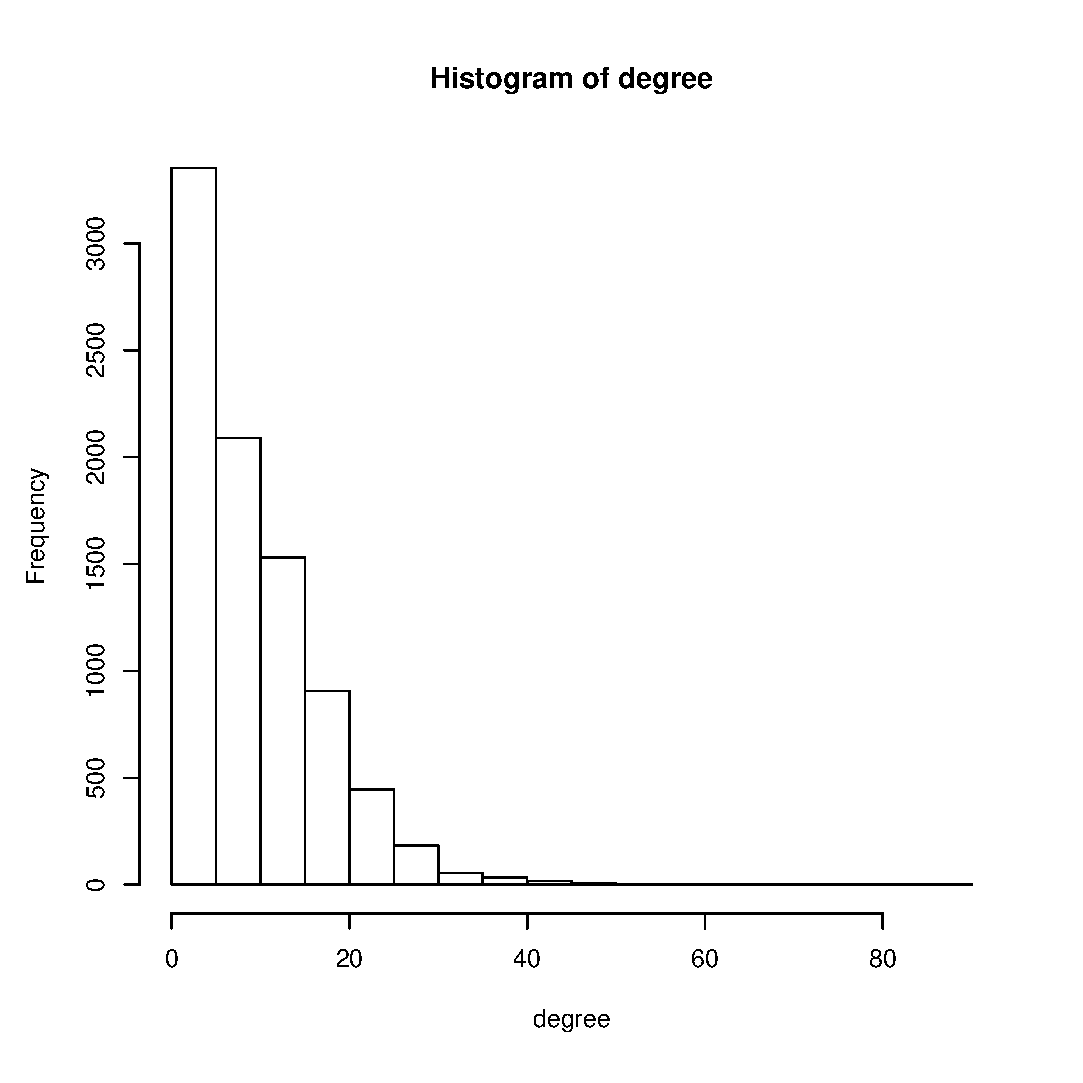
\includegraphics[scale=.5]{degrees.eps}
  \caption{Distribution of \texttt{degree}}
  \label{fig:degrees}
\end{figure}

\begin{figure}
  \centering
  \begin{subfigure}[b]{0.49\textwidth}
    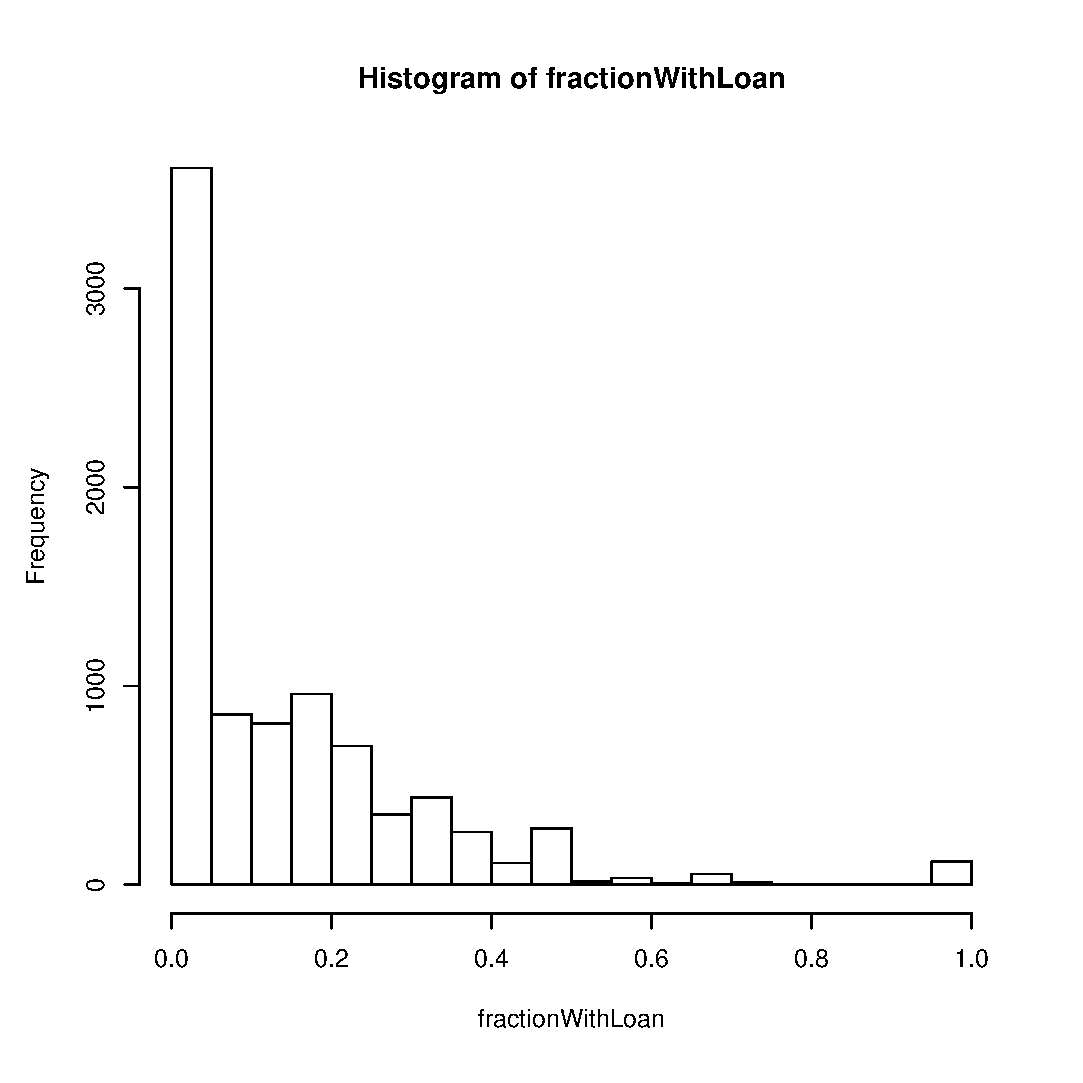
\includegraphics[width=\textwidth]{degrees_frac_with_loan.eps}
    \caption{Distribution of Connected Households with Loans}
    \label{fig:frac_loan}
  \end{subfigure}
  \hfill
  \begin{subfigure}[b]{0.49\textwidth}
    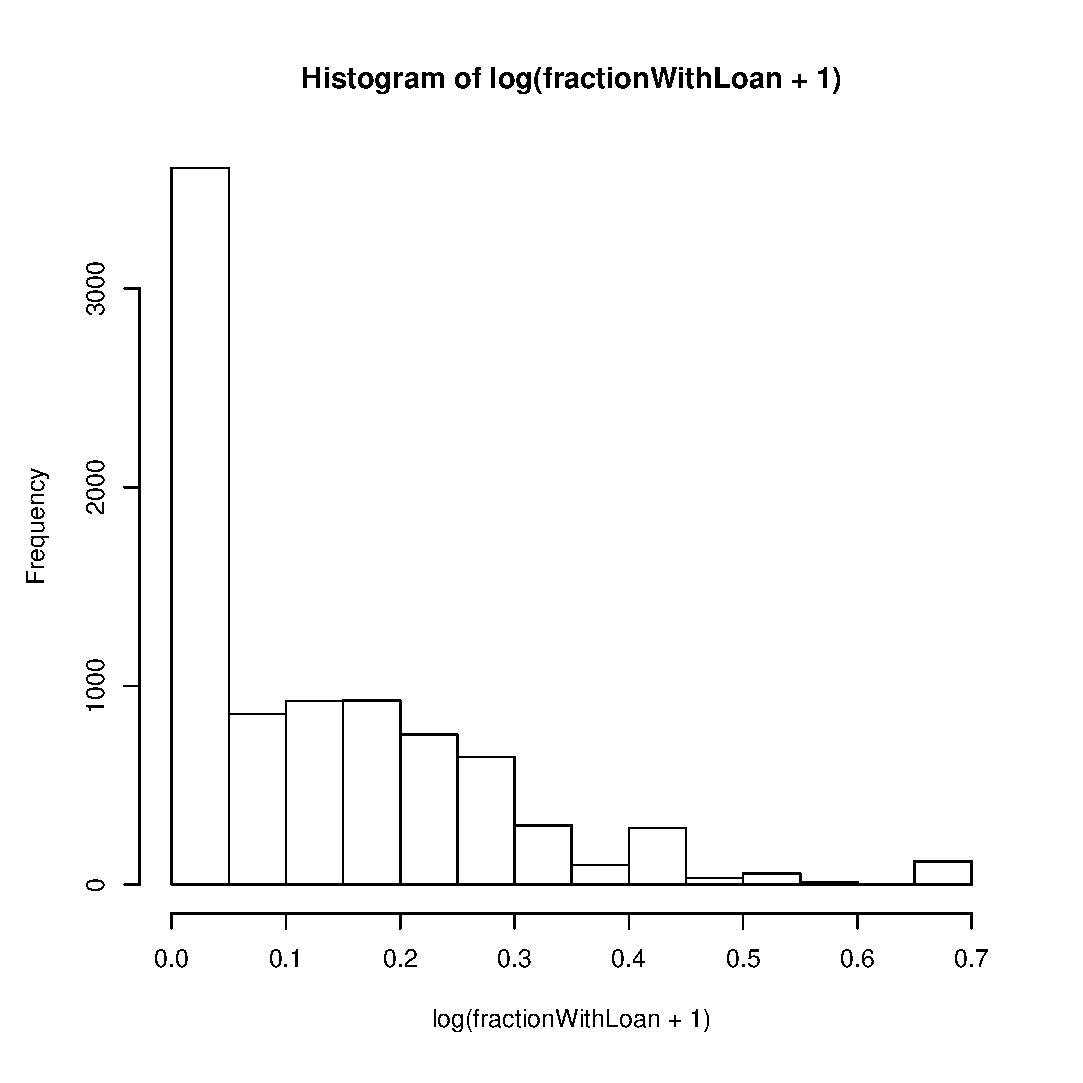
\includegraphics[width=\textwidth]{degrees_frac_with_loan_log.eps}
    \caption{Log Distribution of Connected Network with Loans}
    \label{fig:log_frac_loan}
  \end{subfigure}
  \caption{Normalization of Degree: Fraction of Household's Network with Loans}
\end{figure}

\begin{figure}[!htb]
  \centering
  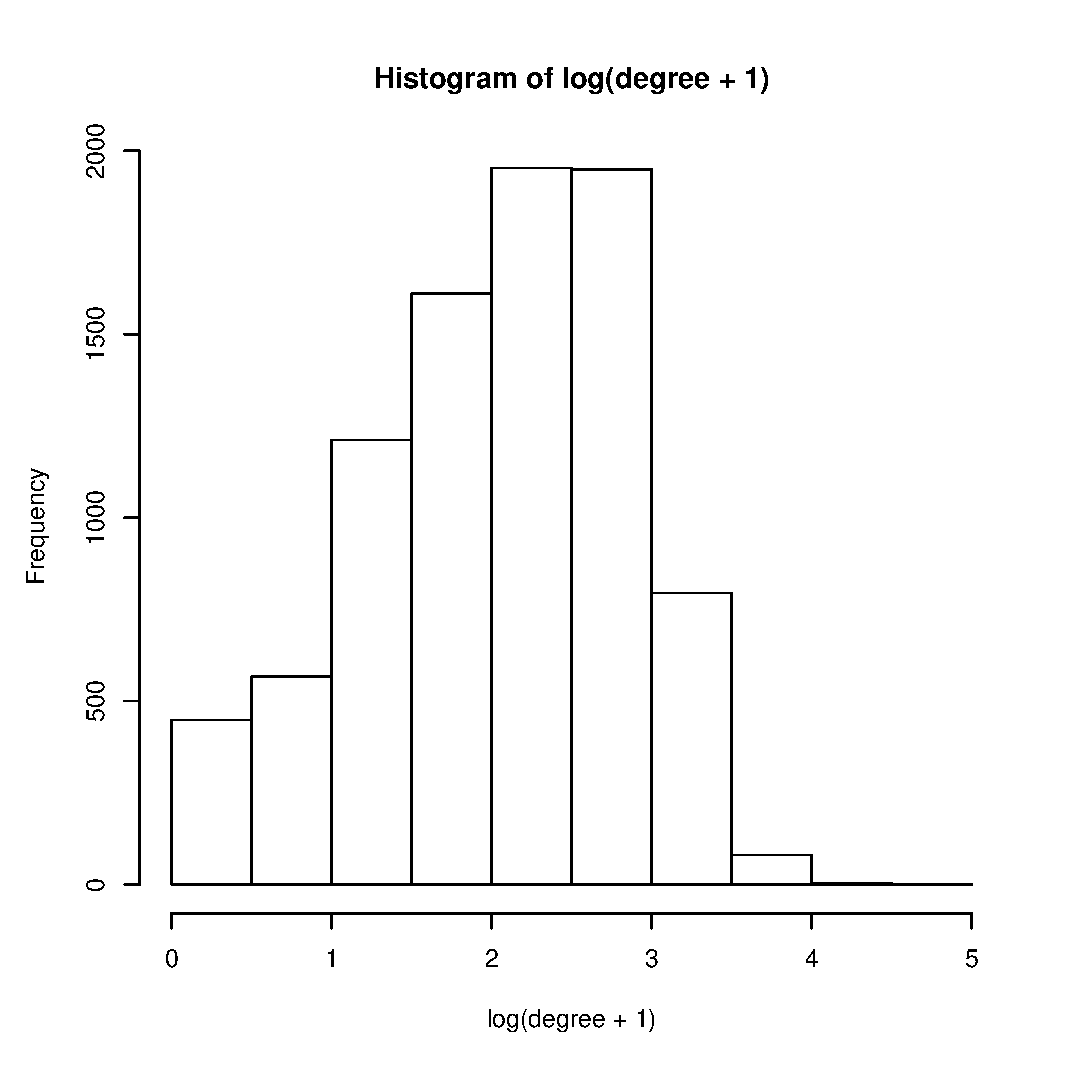
\includegraphics[scale=.5]{degrees_log.eps}
  \caption{Distribution of $\log(\texttt{degree}+1)$}
  \label{fig:log_degrees}
\end{figure}


\section{Predicting Node Connectivity from Controls}
\label{sec:predict}

In this section, we build a model to predict a node's degree by using only our control variables. Our model is: 
\begin{equation} \label{eq:treat}
d(x) = \beta_0 + \bm{X} \bm{\beta} + \nu
\end{equation}

where $d$ is a node's number of degrees, $\bm{X}$ is a vector of control variables including village, religion, type of roof on home, rooms and beds in home, a dummy variable for having electricity in home, whether a home is owned, and whether the person is a ``leader'' in the village. 

We estimate this model using a Gamma-Lasso regression. In Figure~\ref{fig:treat_aic} in the Appendix, we show the Gamma-Lasso path plots with five decision criteria marked: AIC, AICc, BIC, CV.Min, and CV.1se. The $\log(\lambda)$ selected by AICc and by CV.Min are reasonably close to each other (-4.60 and -4.46, respectively, shown in Table~\ref{tab:treat_ic} in the Appendix), which provides us with a confirmation that our model is estimated reasonably well.

We then use the model selected by AICc to predict degree (which we will call $\hat{d}$). We plot $d$ against $\hat{d}$ in Figure~\ref{fig:d_vs_dhat} and see that there is only a very rough correlation between the two ($\sigma_{d,\hat{d}}=0.34$)

\begin{figure}[!htb]
  \centering
  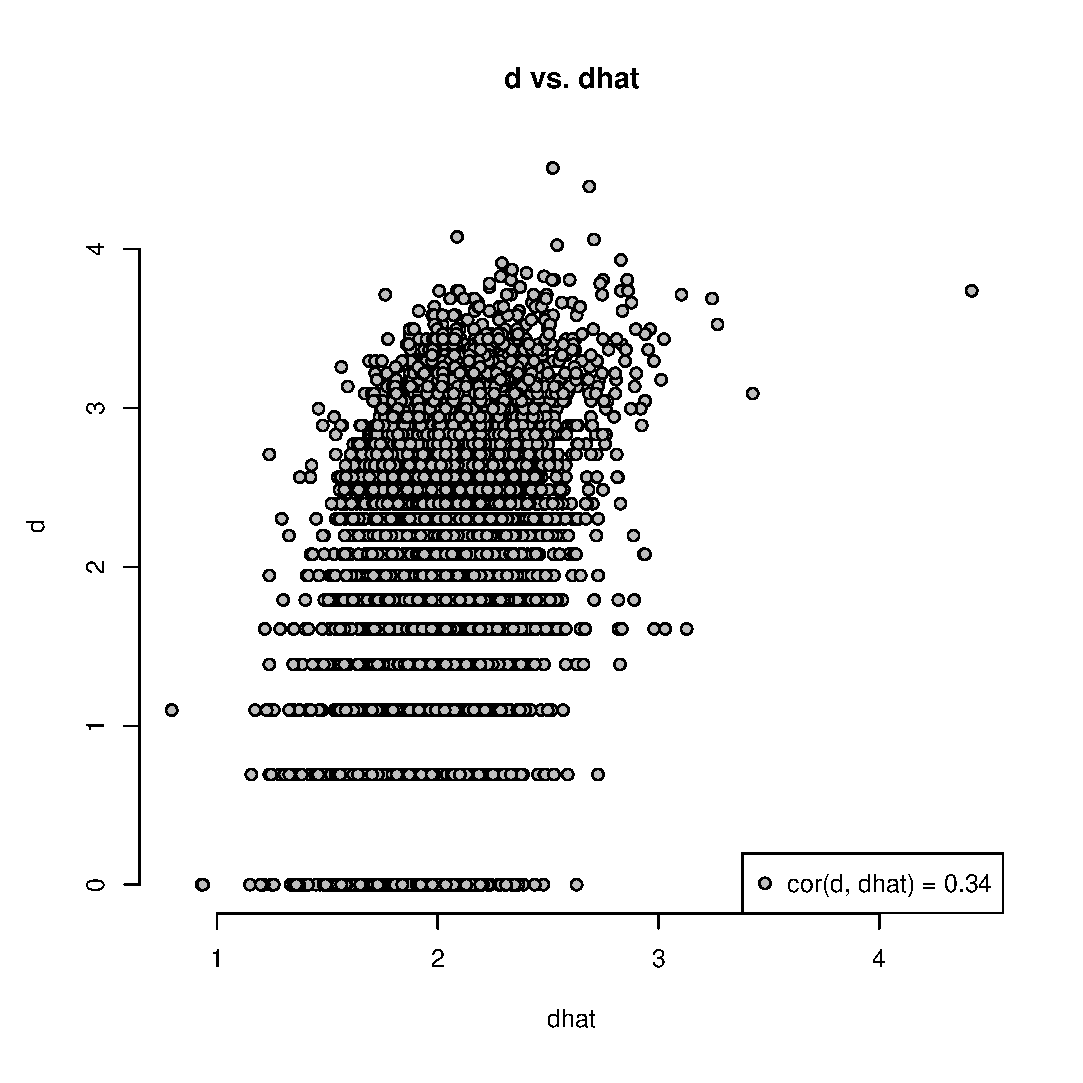
\includegraphics[scale=.5]{d_vs_dhat.eps}
  \caption{Degree and Predicted Degree}
  \label{fig:d_vs_dhat}
\end{figure}

This is a positive result. It tells us that most of the variation in degree, which will be our treatment variable in Section~\ref{sec:model}, is exogenous and cannot be explained by the control variables that we observe. We can therefore measure the effect of degree as a treatment on the propensity to take out a loan and be reasonably sure that we are not simply measuring variation in other observed control variables.

\section{Effect of Node Connectivity on Loan Propensity}
\label{sec:model}

In this section, we use our estimate of predicted degree ($\hat{d}$) to build a model for loan propensity based on node connectivity. We include $\hat{d}$ in our regression model:
\begin{equation} \label{eq:causal}
\log\left(\frac{p}{1-p}\right) = \beta_0 + d \gamma + \hat{d}(x) \delta + \bm{X}\bm{\beta} + \varepsilon
\end{equation}
where $p = \Pr(\text{loan}=1|\bm{X})$. We can substitute in our definition of $\hat{d}(x)$ from equation~\ref{eq:treat}:
\begin{equation}
\log\left(\frac{p}{1-p}\right) = \beta_0 + d \gamma + \left(\beta_0 + \bm{X} \bm{\beta} + \nu\right) \delta + \bm{X}\bm{\beta} + \varepsilon
\end{equation}
which simplifies to
\begin{equation}
\log\left(\frac{p}{1-p}\right) = \beta_0 + \gamma \nu + \hat{d}(x) (\gamma + \delta) + \bm{X}\bm{\beta}
\end{equation}
By estimating the model in equation~\ref{eq:causal}, we can isolate the parameter $\gamma$, which is ultimately the effect of the independent variation in $d$ on the propensity to take out a loan. 

As in Section~\ref{sec:predict}, we use a Gamma-Lasso regression and see that the $\log(\lambda)$ values for the AICc and CV.Min are roughly similar (-5.37 and -5.13, respectively, shown in Table~\ref{tab:causal_ic} and plotted in Figure~\ref{fig:causal_aic} in the Appendix). This tells us our model is reasonably estimated; we proceed using the model chosen by AICc.

The coefficient of interest in this regression is $\gamma$, the effect of exogenous changes in degree connectivity on propensity to take out a loan. In our model, $\gamma$ is 0.0145, which means that having one additional connection (i.e. degree increased by one) increases the odds of taking out a micro-finance loan by 1.46 percent\footnote{$100 \cdot \left( \exp(0.0145) - 1 \right) = 1.46$}. This seems like a reasonable estimate \textemdash the coefficient is small but positive, indicating that knowing more people makes one very slightly more likely to take out a loan. We can imagine a story in which information travels more efficiently to those who are more connected, but it is reasonable to assume that there are much more significant predictors of loan propensity than how many friends a person has.

In Table~\ref{tab:pos} and~\ref{tab:neg}, we see the 5 most positive and negative predictors of loan propensity. At first glance, it appears that there are a few very positive factors that would increase propensity to take out a loan. For example, living in village 4 and having a thatch roof makes one 56.7 percent more likely to have a loan. Upon closer examination, though, there is only one person in our sample in village 4 with a thatch roof, so we cannot infer much from this coefficient. In fact, the top 5 coefficients have sample sizes of $n<5$.

The coefficients in Table~\ref{tab:neg} are more meaningful as the sub-sample sizes are sufficiently large to draw conclusions from. For example, Hindus in village 71 are 4.7 percent less likely to take out a loan. We are sufficiently confident in this coefficient because the sample size of Hindus in village 71 is 252. 

This seems to be one drawback to using a matrix of control factors in which all possible terms interact with each other. In many cases, the Gamma-Lasso regression does not throw out coefficients that we might want to ignore anyway because of sample sizes that are insufficiently large. 

% latex table generated in R 3.0.2 by xtable 1.7-4 package
% Thu Apr 30 17:16:05 2015
\begin{table}[ht]
\centering
\begin{tabular}{rrr}
  \hline
 & $\beta_j$ & odds multiplier \\ 
  \hline
village4:roofthatch & 0.45 & 56.56 \\ 
  village21:ownershipRENTED & 0.42 & 52.63 \\ 
  village3:ownershipSHARE OWNED & 0.41 & 51.01 \\ 
  village65:ownershipLEASED & 0.41 & 50.95 \\ 
  village1:roofthatch & 0.41 & 50.37 \\ 
   \hline
\end{tabular}
\caption{Most Significant Positive Predictors} 
\label{tab:pos}
\end{table}

% latex table generated in R 3.0.2 by xtable 1.7-4 package
% Thu Apr 30 21:28:00 2015
\begin{table}[ht]
\centering
\begin{tabular}{rllll}
  \hline
 & $x$ & $\beta_j$ & $\Delta$ likelihood & n \\ 
  \hline
1 & village50 & -0.0417 & -4.0834 & 244 \\ 
  2 & village59:roofstone & -0.0441 & -4.3095 & 268 \\ 
  3 & village36 & -0.0442 & -4.3231 & 289 \\ 
  4 & village71:religionhindu & -0.0483 & -4.7140 & 252 \\ 
  5 & village20:roofthatch & -0.0903 & -8.6304 & 5 \\ 
   \hline
\end{tabular}
\caption{Most Significant Negative Predictors} 
\label{tab:neg}
\end{table}


\section{Naive Estimation of Loan Propensity}

In this section, run a simple regression of the $\log(odds)$ of obtaining a loan on \texttt{X} and \texttt{d} (see equation~\ref{eq:naive} for the model).  Here we neglect to remove any of the influencers in \texttt{X} (i.e. the rest of the model) that are also correlated with \texttt{d}.

\begin{equation} \label{eq:naive}
\log\left(\frac{p}{1-p}\right) = \beta_0 + d \gamma + \bm{X}\bm{\beta} + \varepsilon
\end{equation}

As in the previous sections, we use a Gamma-Lasso regression.  Here, again, we see that the AICc and the CV.Min are roughly similar (-5.39 and -5.07 respectively, shown in Table~\ref{tab:naive_ic} and plotted in Figure~\ref{fig:naive_aic} in the Appendix).  We do note, perhaps with hindsight bias, that the there is a slightly larger divergence between the choices of $\log(\lambda)$ than in the previous sections.  Using the Gamma-Lasso with the AICc selection criteria, we see that the coefficient ($\gamma$) associated with \texttt{d} is significant and equal to 0.0138.

In terms of odds, each additional connection increases the odds of taking out a loan by 1.39\%\footnote{$100 \cdot \left( \exp(0.0138) - 1\right) = 1.39$}.  This result is very similar from Section~\ref{sec:model} where each connection increased the odds of taking out a loan by 1.46\%.  These vales are similar, but ultimately, differ since some of the effects of \texttt{d} can be predicted by \texttt{X} and have not been controlled for in our model.  It seems that neglecting to control for these confounders may not lead to an outright incorrect answer, but rather to one that is subtly different.  In this case the increase odds differ by each additional connection only differs by 5\%.

\section{Bootstrapping Uncertainty}

In this section, we estimate our uncertainty in the $\gamma$ found in Section~\ref{sec:model} using the bootstrap method.  To accomplish this, we successively take n random samples (with replacement from our data-set), and run the same two regressions discussed in Sections~\ref{sec:predict} \& \ref{sec:model}.  That is, we run a Gamma-Lasso regression and predict each node's degree ($\hat{d}$) and then, using this prediction, run the Gamma-Lasso to determine the effect of \texttt(d) ($\gamma$) on the propensity to obtain a loan.  These sample - regression - prediction - regression steps are performed 100 times; each time, the estimate of $\gamma$ is saved.

From our new estimates of $\gamma$, uncertainty in our original $\gamma$ is measured by finding the standard deviation of the samples.  Figure~\ref{fig:bootstrap_hist} shows a histogram of these $\gamma$'s.  The distribution mean is 0.0168, which is notably different than the one found in Section~\ref{sec:model} (0.0145).  However, with a $\sigma = 0.00422$, the 95\% confidence interval for the unconditional uncertainty in $\gamma$ is $\mu \pm 1.96\sigma = \left[0.00849, 0.0250\right]$, which easily contains our previous estimate.  In terms of $\log(\text{odds})$ this confidence interval concludes that each additional degree of connection corresponds to a lift between $\left[0.852\%, 2.53\%\right]$ in the odds of obtaining a loan.  This range quite a bit higher than we would have previously guessed and seems to suggest that the degree of household connectedness isn't the best predictor of loan propensity.

%gamma mean=0.016760, std-dev=0.004221
%mean(gamma)+1.96*sqrt(var(gamma))
%[1] 0.02503385
%> mean(gamma)-1.96*sqrt(var(gamma))
%[1] 0.008486115
%100 * (exp(0.008486115)-1)
%[1] 0.8522224
%> 100 * (exp(0.02503385)-1)
%[1] 2.534983
%> 100 * (exp(0.0168)-1)
%[1] 1.694191

\begin{figure}[!htb]
  \centering
  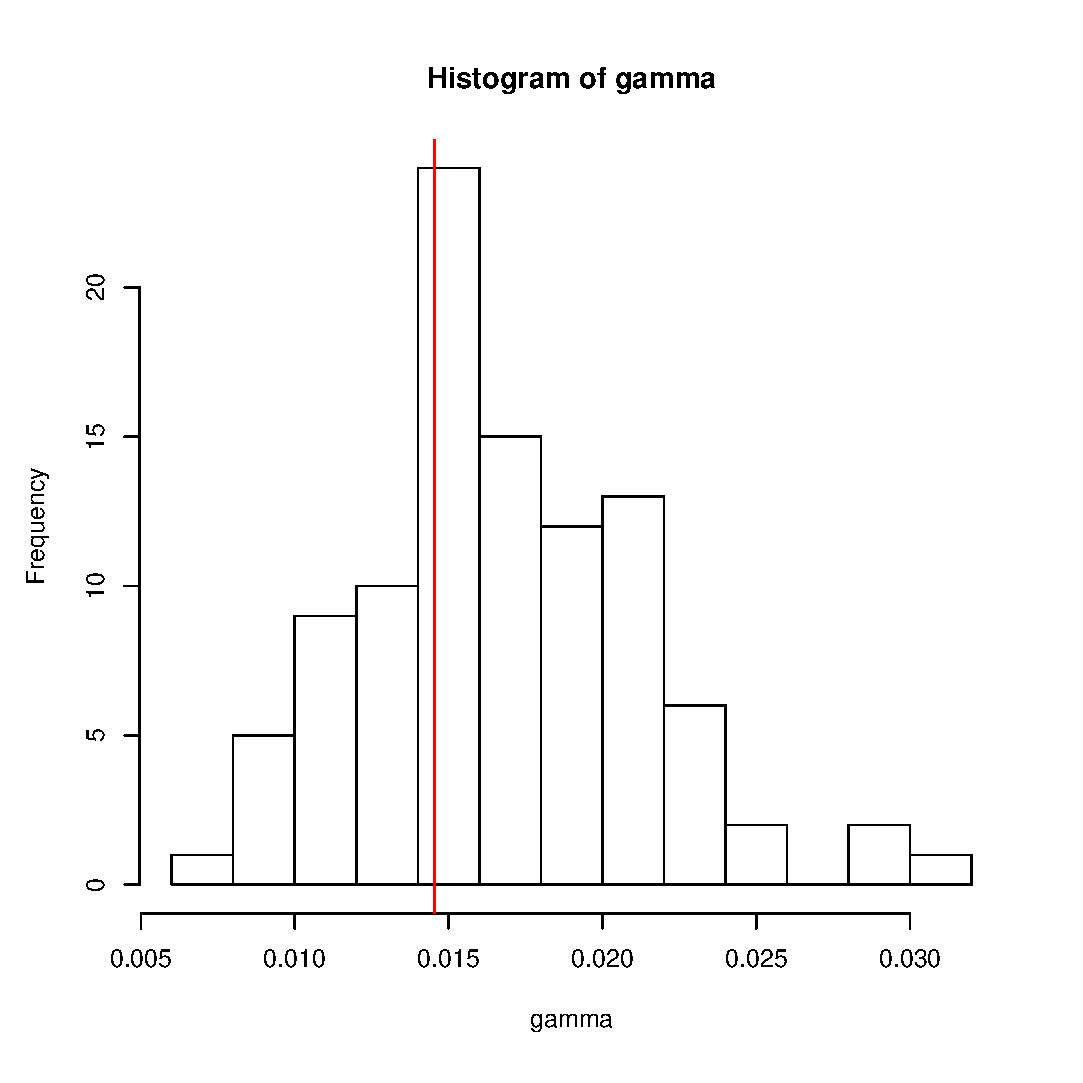
\includegraphics[scale=.5]{bootstrap_hist.eps}
  \caption{Distribution of $\gamma$ via Bootstrap Method (k=100)}
  \label{fig:bootstrap_hist}
\end{figure}

\section{Experimental Design}

Since degrees of connectedness amongst households are primarily observables, it is difficult to truly design an experiment to better estimate the treatment effect. However, one could, perhaps, setup an experiment whereby households in the treatment group are introduced by the experimenters to people they are currently unconnected to.  Likewise households in the control group are left alone.  If there is a noticeable lift in the propensity to obtain a loan in the treatment group, versus the control group, then one could possibly establish the effect of the degree of connectedness from the experiment.

\section{Appendix}

\begin{figure}[!htb]
  \centering
  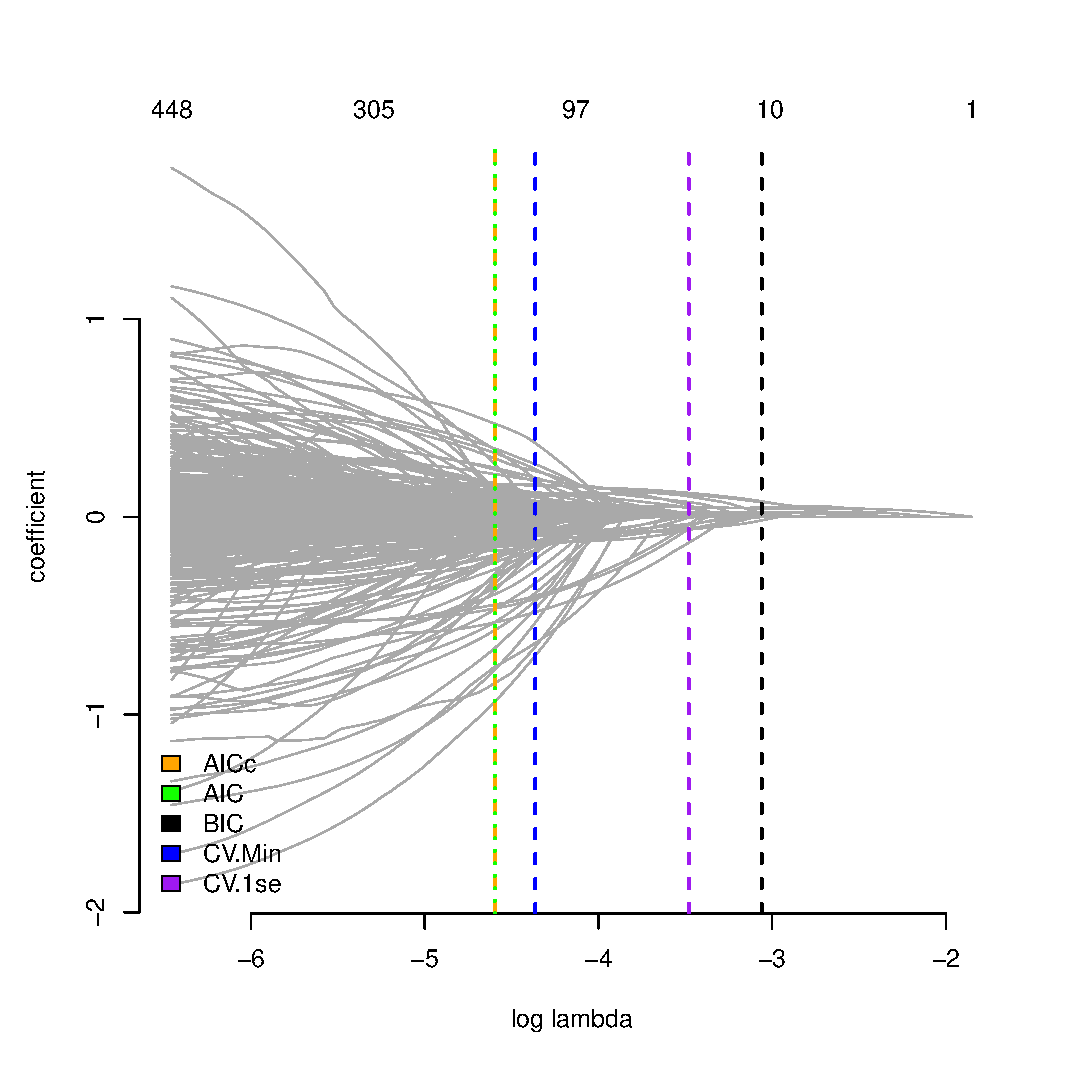
\includegraphics[scale=.5]{treat_aic.eps}
  \caption{Gamma-Lasso Regression for Degree on Controls}
  \label{fig:treat_aic}
\end{figure}

% latex table generated in R 3.0.2 by xtable 1.7-4 package
% Thu Apr 30 15:31:29 2015
\begin{table}[ht]
\centering
\begin{tabular}{rrr}
  \hline
 & $\log(\lambda)$ & Covariates Selected \\ 
  \hline
AICc & -4.60 & 185 \\ 
  AIC & -4.60 & 185 \\ 
  BIC & -3.06 &  10 \\ 
  CV.Min & -4.46 & 161 \\ 
  CV.1se & -3.53 &  37 \\ 
   \hline
\end{tabular}
\caption{Treatment IC Table} 
\label{tab:treat_ic}
\end{table}


\begin{figure}[!htb]
  \centering
  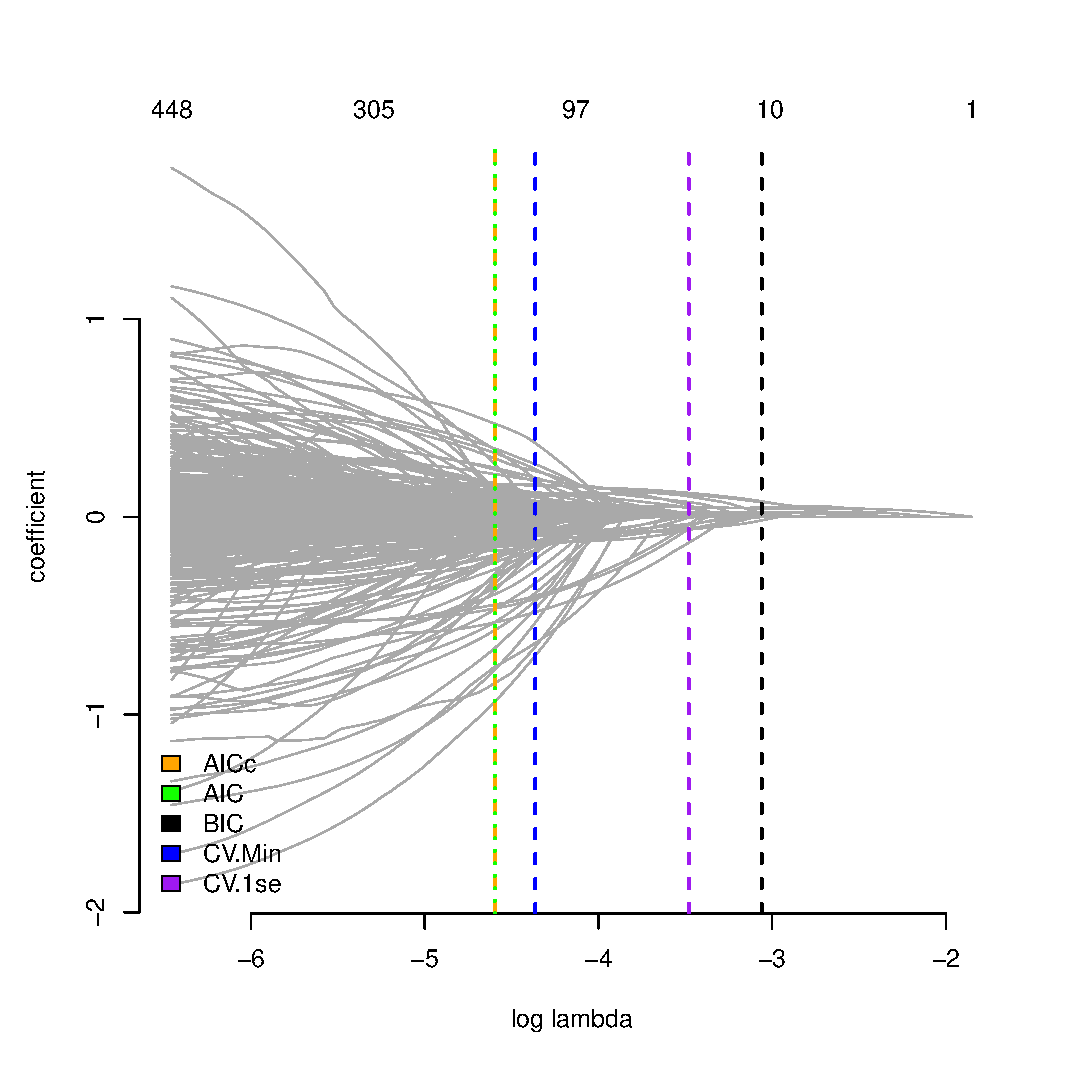
\includegraphics[scale=.5]{treat_aic.eps}
  \caption{Gamma-Lasso Regression for Loan Propensity on Degree}
  \label{fig:causal_aic}
\end{figure}

% latex table generated in R 3.1.2 by xtable 1.7-4 package
% Wed Apr 29 22:13:10 2015
\begin{table}[ht]
\centering
\begin{tabular}{rrr}
  \hline
 & $\log(\lambda)$ & Covariates Selected \\ 
  \hline
AICc & -5.37 & 148 \\ 
  AIC & -5.37 & 148 \\ 
  BIC & -3.97 &  12 \\ 
  CV.Min & -5.13 & 116 \\ 
  CV.1se & -3.60 &   2 \\ 
   \hline
\end{tabular}
\caption{Causal IC Table} 
\label{tab:causal_ic}
\end{table}


\begin{figure}[!htb]
  \centering
  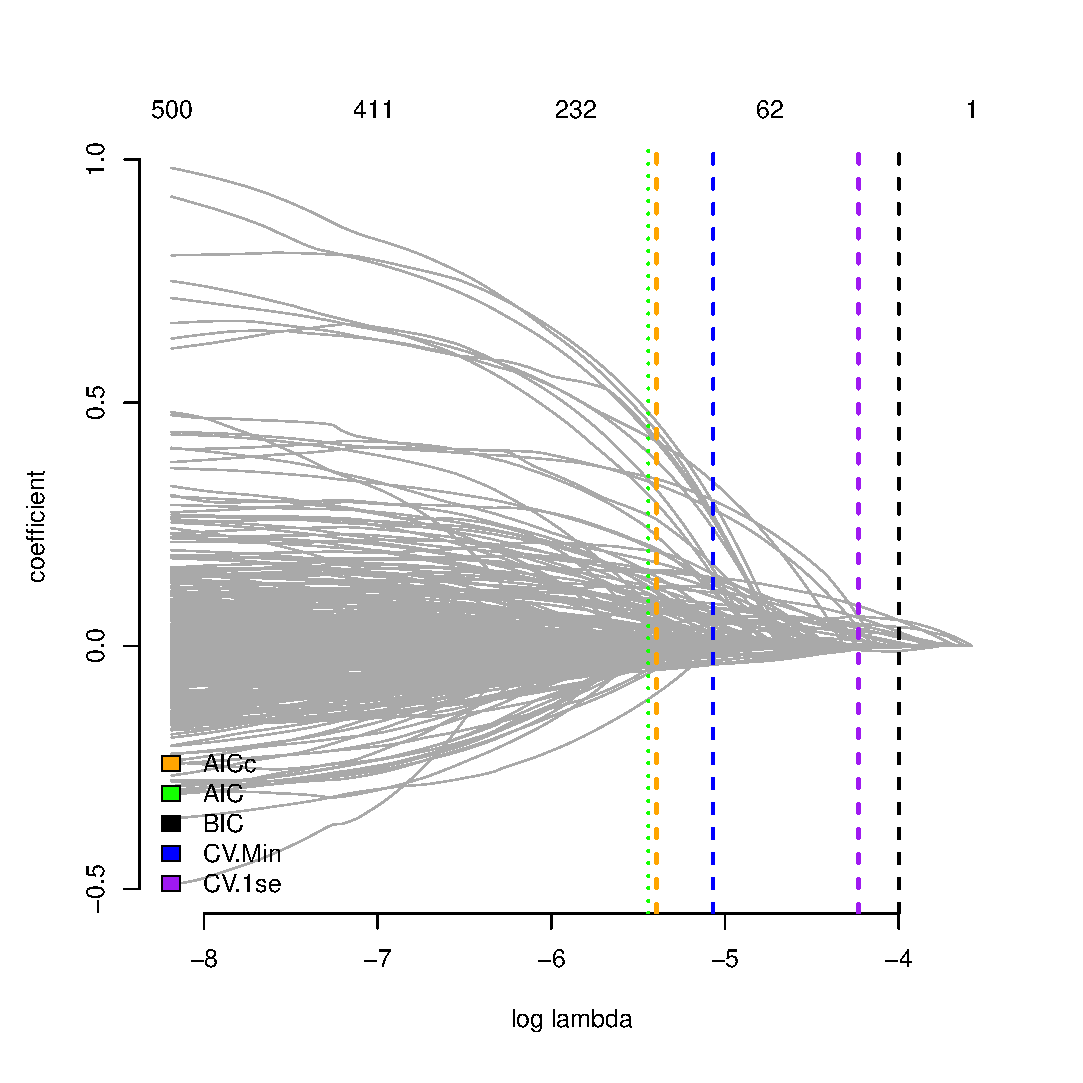
\includegraphics[scale=.5]{naive_aic.eps}
  \caption{Gamma-Lasso Regression for Naive Loan Propensity}
  \label{fig:naive_aic}
\end{figure}

% latex table generated in R 3.1.2 by xtable 1.7-4 package
% Wed Apr 29 22:13:14 2015
\begin{table}[ht]
\centering
\begin{tabular}{rrr}
  \hline
 & $\log(\lambda)$ & Covariates Selected \\ 
  \hline
AICc & -5.39 & 151 \\ 
  AIC & -5.44 & 159 \\ 
  BIC & -4.00 &  14 \\ 
  CV.Min & -5.07 & 105 \\ 
  CV.1se & -4.23 &  26 \\ 
   \hline
\end{tabular}
\caption{Naive IC Table} 
\label{tab:naive_ic}
\end{table}



\end{document}
